\documentclass[a4paper,12pt]{article}
\usepackage{blindtext}
\usepackage[utf8]{inputenc}
\usepackage{graphicx}
\usepackage{enumitem}
\usepackage{booktabs}
\usepackage{verbatim}
\usepackage{makecell}

\begin{document}
\begin{titlepage}
\center

\textsc{\LARGE Testing Documentation}\\[1.5cm]
\textsc{\Large Project: Traffic Camera Image Analysis}\\[1.5cm]
\textsc{\large Client: DPSS, CSIR}\\[0.5cm]
\textsc{\large Team: Quadcore Productions}\\[0.5cm]

\begin{minipage}{0.4\textwidth}
\begin{flushleft} \large
\textbf{Author(s):}\\
Mpho \textsc{Baloyi}\\
Hlengekile \textsc{Jita}\\
Mayimela \textsc{Moses}\\
Mbhele \textsc{Themba}\\
\end{flushleft}
\end{minipage}
~
\begin{minipage}{0.4\textwidth}
\begin{flushright} \large
\textbf{Student number(s):} \\
14133670\\ % Student number
14077893\\
14019702\\
14007950\\
\end{flushright}
\end{minipage}\\

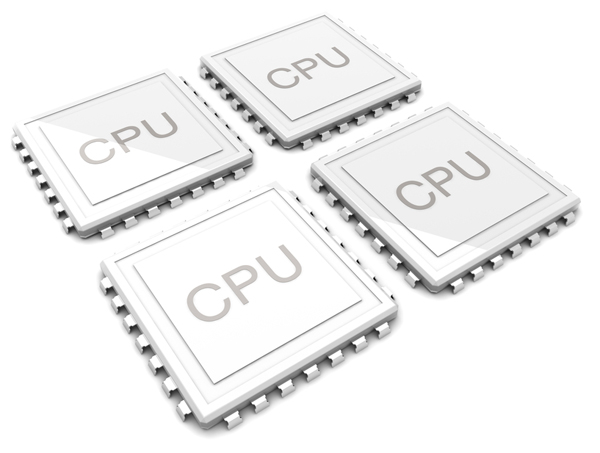
\includegraphics[width=\textwidth]{2012-quad-core-phones.jpg}

{\large University of Pretoria, Department of Computer Science}\\

{\large 29 July 2016}\\[3cm]

\vfil

\end{titlepage}

\newpage
\tableofcontents
\newpage

\newpage
%\begin{comment}
\begin{table}[ht]
 \centering
 \caption{Version History}
 \label{tab:table1}
 \begin{tabular}{cccc}
   \toprule Version No. & Date & Changes & By\\
   \midrule 1 & 29 July 2016 & & \makecell {Mpho Baloyi,\\ Hlengekile Jita,\\ Moses Mayimela,\\ Themba Mbhele}\\
   \bottomrule
  \end{tabular}
\end{table}
%\end{comment}
\newpage

\section{Introduction}
This document contains the testing methods that we have used to test the Traffic Camera Image Analysis system that we are currently developing for our final project for COS301 project. We will document the tests that are currently in place and have been run, and future tests that we still plan to design as we continue to develop the system.

\section{Plan for Testing (Android)}
\subsection{Testing tools}
As the functions that are being used by the system were developed, tests were designed to test their functionality to verify that the functions do what they are intended to do so that as we continue with the development, we use functions that have been thoroughly tested and have been verified as correct.
On the android side of the system, JUnit was used to conduct all unit tests. We
made use of a testing framework because it allows us to automate the testing process because we do not have to manually run tests for each function that we intend to test, instead JUnit will run all of the tests for us provided that we
have properly annotated our functions and made use of assertions.
\subsection{Running the unit tests}
To run the unit test for Android, an internet connection has to be established and an IDE such as eclipse, android studio or IntelliJ must be used. Once that infrastructure is in place, and the tests have all been written, executing the tests simply involves right clicking on the folder in which the unit tests are located and choosing the "run tests" options. this will execute all the tests in that folder and generate a report displaying the results of the tests.
\subsection{Plans for the future}
Once the application has been completed, we plan to conduct usability tests where we gather a number of people to test the application. The aim of these tests will be to determine whether the user interface of the application is user friendly and the test will also reveal any flaws in the system
\section{Plan for Testing (Server)}
\subsection{getImages.py}
To test the script, the following must be met
\begin{itemize}
\item Python version 2.7
\item There must be a folder with the name "traffic\_images"
\item The computer where the script will be tested should have an internet connection
\item Mysql server
\item If Possible, you may verify if the itraffic website is operational.
\item This script was written and tested on a UNIX environment and this is the environment where it should be tested.
\item The "TrafficAnalyzer" Django project should be in the same folder as the "getImages.py". This is becauset the script makes use of the files in the Django project.
\end{itemize}

After the above requirements have been met,the script can be manually executed on the terminal or it may be executed.

\subsection{Django project}
The Django project will handle all the requests from the android device regarding camera information. The following is a list of the requirements for the Django application to work.
\begin{itemize}
\item Mysql server 5.6 or above
\item Django 1.7.6
\item python-mysql connector
\item The project was developed in a UNIX environment.
\item The server should have an internet connection.
\item The port where the server is listening should be enabled. E.g 8000.
\item The website also works with information form the itraffic website and thus it should be verified that the itraffic website is active to avoid avoid incorrect results from the server.
\end{itemize}
To Test the server, an Android device or a web browser may be used to send requests to the django application. Then the application should be able to respond with relevant information. Giving it known latitude-longitude combination and verify if the cameras returned are correct.
\end{document}
